\section{Theory}
Almost all solids with the exception of amorphous solids and glasses have periodic arrays of atoms which form a crystal lattice. The existence of the periodic crystal lattice in solid materials provides a medium for characteristic vibrations. Between the lattice spacing, there are quantized vibrational modes called a phonon. The study of phonon is an important part of solid state physics, as they play an essential role in the physical properties of solids, the thermal and electrical conductivity of the materials. The long wavelength property of phonon also gives attributes to sounds in solids.

\subsection{Monoatomic One Dimensional Lattice}
Consider the mono-atomic 1D crystal lattice. It can be modelled with an infinite spring mass system with particles having mass $m$ connected by spring constant $f$. The equilibrium distance between the particles is $a$. Assuming only the nearest neighbour interaction, the equation of motion of the $n$-th atom is given by,

\begin{figure}
    \centering
    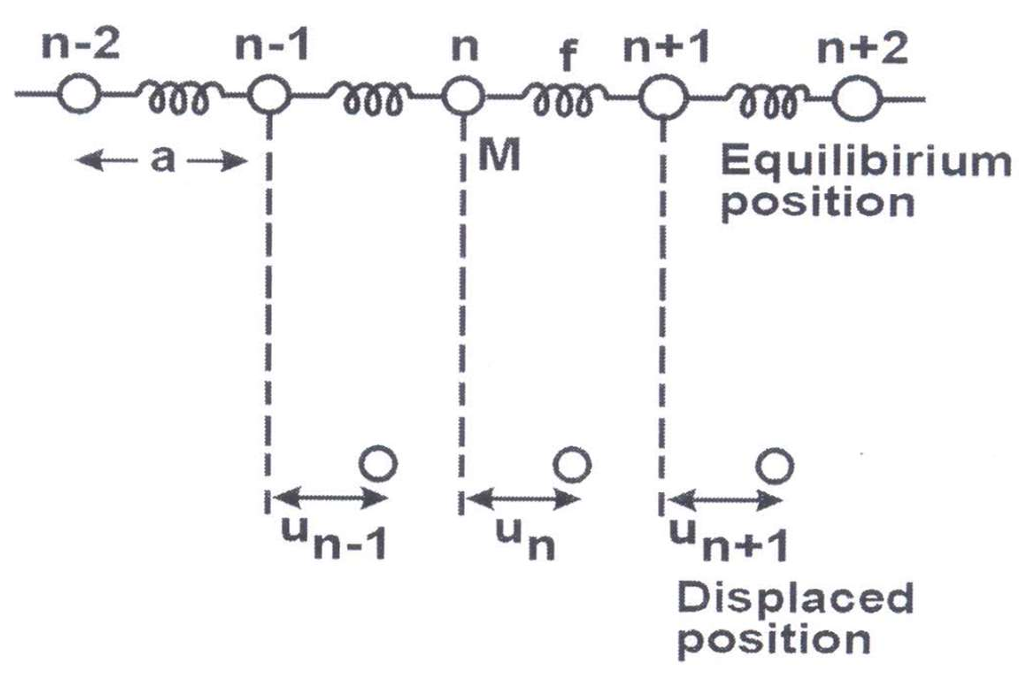
\includegraphics[width=.8\columnwidth]{images/theory2.png}
    \caption{A one-dimensional monoatomic lattice}
    \label{f1}
\end{figure}

\begin{align}
    m\frac{d^2U_n}{dt^2} = f(U_{n+1}-U_{n-1} - 2U_n)
\end{align}

\noindent which when solved gives the angular frequency,

\begin{align}
    \omega = \sqrt{\frac{2f}{m}(1-\cos \theta)}
\end{align}    

where, $\theta = ka$ is the phase change per unit cell. The above equation shows that there exists a maximum frequency
\begin{align}
    \nu_\text{max} = \frac{\omega_\text{max}}{2\pi} = \frac{1}{\pi}\sqrt{\frac{f}{m}}
\end{align}

beyond which no transmission occurs. The array may be considered as a low-pass filter which transmits only in the range $0$ to $\nu_\text{max}$.

% ======================================================================
\subsection{Diatomic One Dimensional Lattice}
\begin{figure}[H]
    \centering
    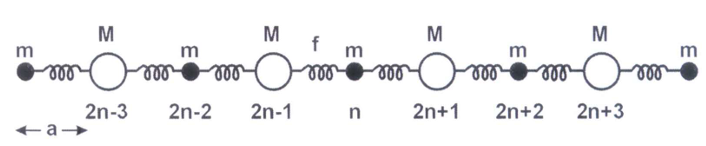
\includegraphics[width=1\columnwidth]{images/theory3.png}
    \caption{A one-dimensional diatomic lattice}
    \label{f2}
\end{figure}
The spring-mass analogy of di-atomic lattice can be given by assuming two different masses connected by springs in series alternatively. For di-atomic lattice we can use same spring-mass formulation to find as a function of phase angle.

\begin{align}
    m_1\frac{d^2U_{2n}}{dt^2} &= f(U_{2n+1}-U_{2n-1} - 2U_{2n})\\
    m_2\frac{d^2U_{2n+1}}{dt^2} &= f(U_{2n+2}-U_{2n} - 2U_{n+1})
\end{align}

Solving for $U_{2n}$ and $U_{2n+1}$ by taking,

\begin{align}
    U_{2n} = Ae^{-i\omega t-2ikna} \text{ and } U_{2n+1} = Be^{-i\omega t-2ikna}
\end{align}

we get an eigenvalue equation, where $k$ is the wavenumber, $\omega$ is the angular frequency and $a$ is the distance between two atoms on the chain. On solving for $\omega$, we get 

\begin{align}
    % \omega^2 &= f\left(\frac{1}{m_1}+\frac{1}{m_2}\right) \pm C \left[\left(\frac{1}{m_1}+\frac{1}{m_2}\right)^2 - \frac{4\sin^2 \theta}{m_1m_2}\right]^{1/2}\\
    \omega^2_{\pm} &= \frac{f}{mM}\left[m+M\pm \sqrt{(m-M)^2+4mM\cos^2(ka)}\right] 
\end{align}

The resulting dispersion relation is sketched in Fig. \ref{f3} for the first Brillouin zone (where $k \in [-\pi/2a, \pi/2a)$).
Note that there is a gap in the spectrum on the boundary of the Brillouin zone, $k = \pm \pi/2a$, given by

\begin{align}
    \Delta E = \hbar \sqrt{2f} \left|\frac{1}{\sqrt{m}}-\frac{1}{\sqrt{M}}\right|
\end{align}

Thus, in a diatomic lattice, where two different atomic species alternate, the frequency spectrum divides into two distinct branches --

\begin{itemize}
    \item The \textbf{acoustic branch} which is characterized by low-frequency oscillations where adjacent atoms move in unison. It os called so because its dispersion relation is of the form $\omega= ck$ characteristic of sound waves, at small $k$.
    \item and the \textbf{optical branch} which is characterized by by high-frequency oscillations where adjacent atoms oscillate out of phase. It is called so because the long wavelength optical modes in ionic crystals can interact with electromagnetic radiation, and are responsible for much of the characteristic optical behavior of such crystals.\\
\end{itemize}

Hence a bandgap, emerges between these
branches, prohibiting wave propagation with certain energies.

\begin{figure}
    \centering
    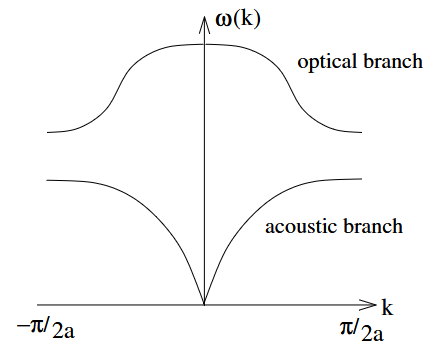
\includegraphics[width=.8\columnwidth]{images/th1.png}
    \caption{Phonon dispersion relation for a diatomic chain.}
    \label{f3}
\end{figure}


% ======================================================================
\subsection{The Electrical Analogue of Lattice Vibrations}
The point is that both the LC circuit and a lattice of atoms (in the limit of small displacements) are harmonic oscillators, and as such, they obey similar dynamics. With just change the symbols to go from one system to the other, but the equations of motion are formally the same.

The dispersion relation for the electrical analogue circuit for monoatomic lattice is

\begin{align}
    \omega_\text{mono} = \sqrt{\frac{2}{LC}(1-\cos \theta)}
\end{align}

Here, the highest possible frequency in the circuit will be 

\begin{align} \label{wf}
    \omega_\text{max} = \frac{2}{\sqrt{LC}}
\end{align}

In the analogy, inductance $L$ represents the atomic mass $m$ and the reciprocal of capacitance $1/C$ represents the force constant $f$.

\begin{figure}[H]
    \centering
    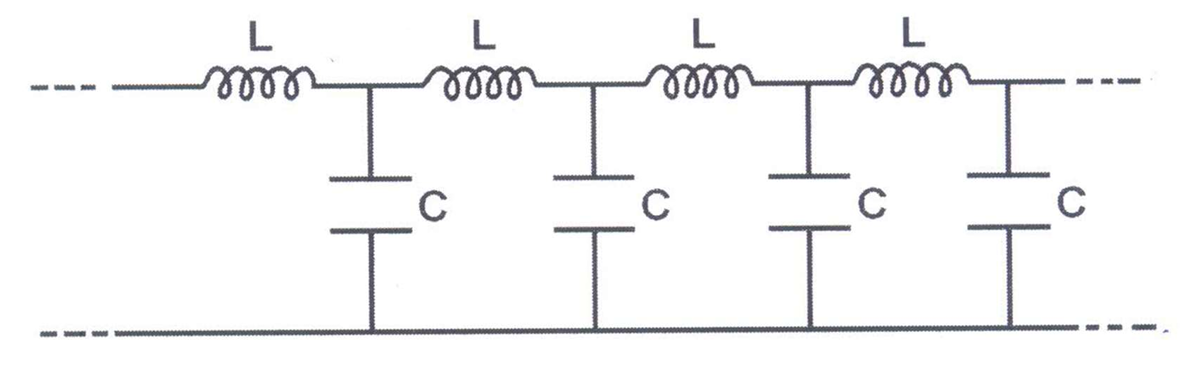
\includegraphics[width=1\columnwidth]{images/circ1.png}
    \caption{Circuit diagram representing a monoatomic lattice with $L$ and $C$}
    \label{c1}
\end{figure}

\begin{figure}[H]
    \centering
    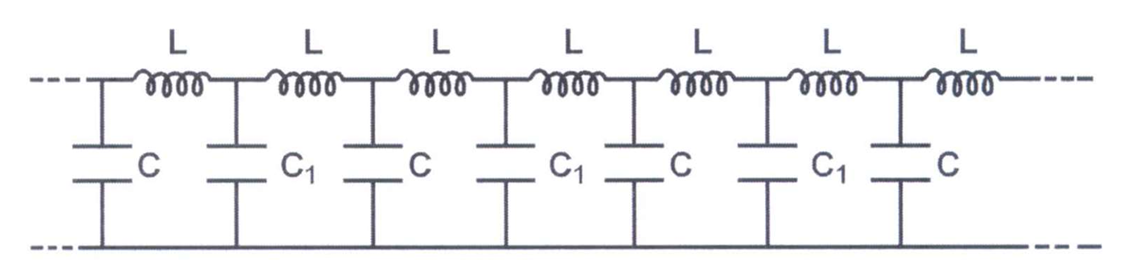
\includegraphics[width=1\columnwidth]{images/circ2.png}
    \caption{Circuit diagram representing a diatomic lattice with $L$ and two values of capacitance $C_1$ and $C_2$}
    \label{c2}
\end{figure}


Here, the bandgap is represented by a frequency gap, prohibiting wave propagation in a certain
frequency range. The electrical circuit analogy enables
controlled tuning of the bandgap by adjusting component
values. The dispersion relation for the electrical analogue
circuit for diatomic lattice is

\begin{align}
    \omega_\text{di}^2 = \frac{1}{L}\left(\frac{1}{C_1}+\frac{1}{C_2}\right) \pm \frac{1}{L} \left[\left(\frac{1}{C_1}+\frac{1}{C_2}\right)^2 - \frac{4\sin^2 \theta}{C_1C_2}\right]^{1/2}
\end{align}

Thus the frequency gap for the diatomic lattice system is the difference between the minimum optical frequency and the maximum acoustic frequency, given by,

\begin{align} \label{wf2}
    f_\text{gap} = \frac{1}{2\pi}\sqrt{\frac{2}{LC_1}} - \frac{1}{2\pi}\sqrt{\frac{2}{LC_2}}
\end{align}

When the alternating elements in a diatomic lattice become identical, the system behaves as a monoatomic lattice, leading to a continuous frequency spectrum without a bandgap.

% \subsubsection*{Optical and Acoustic Branches}

% ======================================================================
\section{Experimental Setup}
The circuit diagrams used in the experiment are shown in Fig. \ref{c1} and \ref{c2}.

\subsection*{Apparatus}

\begin{enumerate}
    \item Inductors
    \item Capacitors with 2 different values
    \item Signal generator
    \item Oscilloscope
    \item Breadboard
    \item DC Power Supply
    \item Connecting Wires
    \item Multimeter and LCR Multimeter
\end{enumerate}
